\chapter{PENDAHULUAN}
\label{bab:1}

\section{Latar Belakang}
Di era industri modern, tuntutan terhadap sistem manufaktur dan otomatisasi
berpresisi tinggi bergerak selaras dengan kebutuhan optimasi performa mesin.
Perangkat berbasis kendali posisi, seperti mesin \textit{Computer Numerical
Control} (CNC), robot lengan industri, hingga mesin pengemasan otomatis, sangat
bergantung pada keandalan sistem penggerak aktuator posisi. Motor servo AC
merupakan aktuator standar yang paling banyak digunakan pada lini produksi
berskala industri karena keunggulannya dalam menghasilkan torsi yang konstan,
kecepatan tinggi, serta umpan balik posisi yang instan melalui sistem
\textit{encoder}. Salah satu sistem penggerak servo industri yang memiliki rekam
jejak keandalan tinggi adalah \textit{Servo Amplifier} Mitsubishi
Melservo-J2-Super (MR-J2S-10A). Namun, akurasi penargetan posisi dan ketahanan
fisik komponen mekanis transisi tidak hanya ditentukan oleh spesifikasi
perangkat keras motor servo itu sendiri, melainkan sangat dipengaruhi oleh
kualitas algoritma \textit{trajectory planning} (perencanaan lintasan) yang
tertanam pada sistem kendali.

\begin{figure}[htbp]
    \centering
    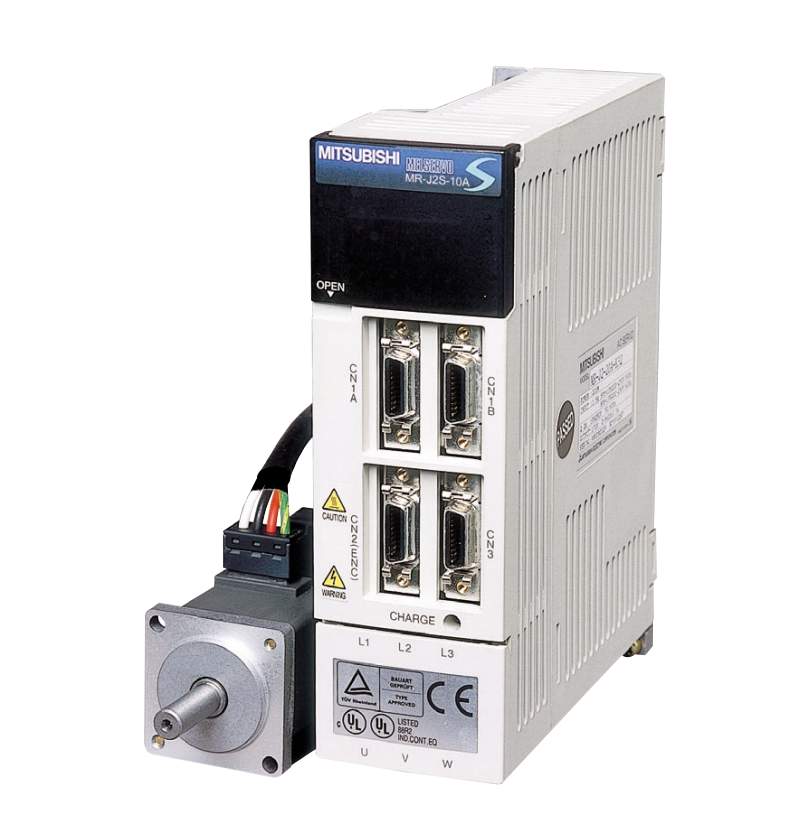
\includegraphics[width=0.27\textwidth]{Gambar/ServoAmp.png}
    \caption{Servo Amplifier Mitsubishi MR-J2S-10A}
    \label{fig gambar_bab1}
\end{figure}

Pada praktiknya, standar aplikasi industri modern umumnya mengadopsi profil
pergerakan \textit{trapezoidal} (percepatan linier) untuk mengontrol akselerasi
dan deselerasi aktuator \parencite{schnegas2024trajectory}. Walaupun laju
kecepatannya berangsur konstan, profil \textit{trapezoidal} memiliki cacat
matematis mendasar berupa perubahan percepatan yang diskontinu pada titik-titik
transisi sudut kurva kecepatan. Ketidakkontinuan ini menghasilkan nilai sentakan
mekanis (\textit{jerk}) yang tak terhingga pada setiap titik belok kurva. Di
sisi lain, profil pergerakan \textit{rectangular} (kecepatan konstan) merupakan
metode tanpa kontrol kelenturan di mana motor dipaksa melompat dari kondisi diam
menuju kecepatan penuh secara instan. Penerapan profil \textit{rectangular} di
industri modern dianggap sebagai kegagalan desain karena memicu lonjakan arus
listrik (\textit{current spike}) yang ekstrem serta benturan mekanis yang
destruktif. Meski demikian, profil \textit{rectangular} tetap diikutsertakan
dalam penelitian ini murni sebagai pembanding batas bawah \textit{(worst-case
baseline)} untuk mengukur kuantitas anomali gerakan jika sistem berjalan tanpa
perencanaan lintasan.

Pada sistem mekanis nyata yang memiliki fleksibilitas dan keterbatasan inersia,
seperti sistem transmisi \textit{linear ball screw} yang terdapat pada modul
laboratorium ED4270m, nilai \textit{jerk} yang tinggi pada transisi gerak memicu
timbulnya getaran sisa (\textit{residual vibration}) yang parah. Getaran
tersebut tidak hanya memperpanjang durasi waktu pemantapan posisi
(\textit{settling time}) aktuator untuk mencapai kondisi benar-benar diam
(\textit{steady state}), melainkan juga mempercepat keausan fisik komponen
kritis seperti \textit{ball screw} dan \textit{bearing}. Untuk menanggulangi
fenomena osilasi tersebut, algoritma \textit{S-Curve trajectory planning}
berorde tiga diterapkan. Profil \textit{S-Curve} membatasi nilai \textit{jerk}
pada batas konstan tertentu sehingga kurva percepatan naik secara landai
membentuk kurva halus menyerupai huruf ``S''. Hal ini memastikan transisi gaya
mekanis di dalam komponen berjalan mulus dan mengeliminasi eksitasi getaran
frekuensi tinggi pada struktur mekanis.

\begin{figure}[htbp]
    \centering
    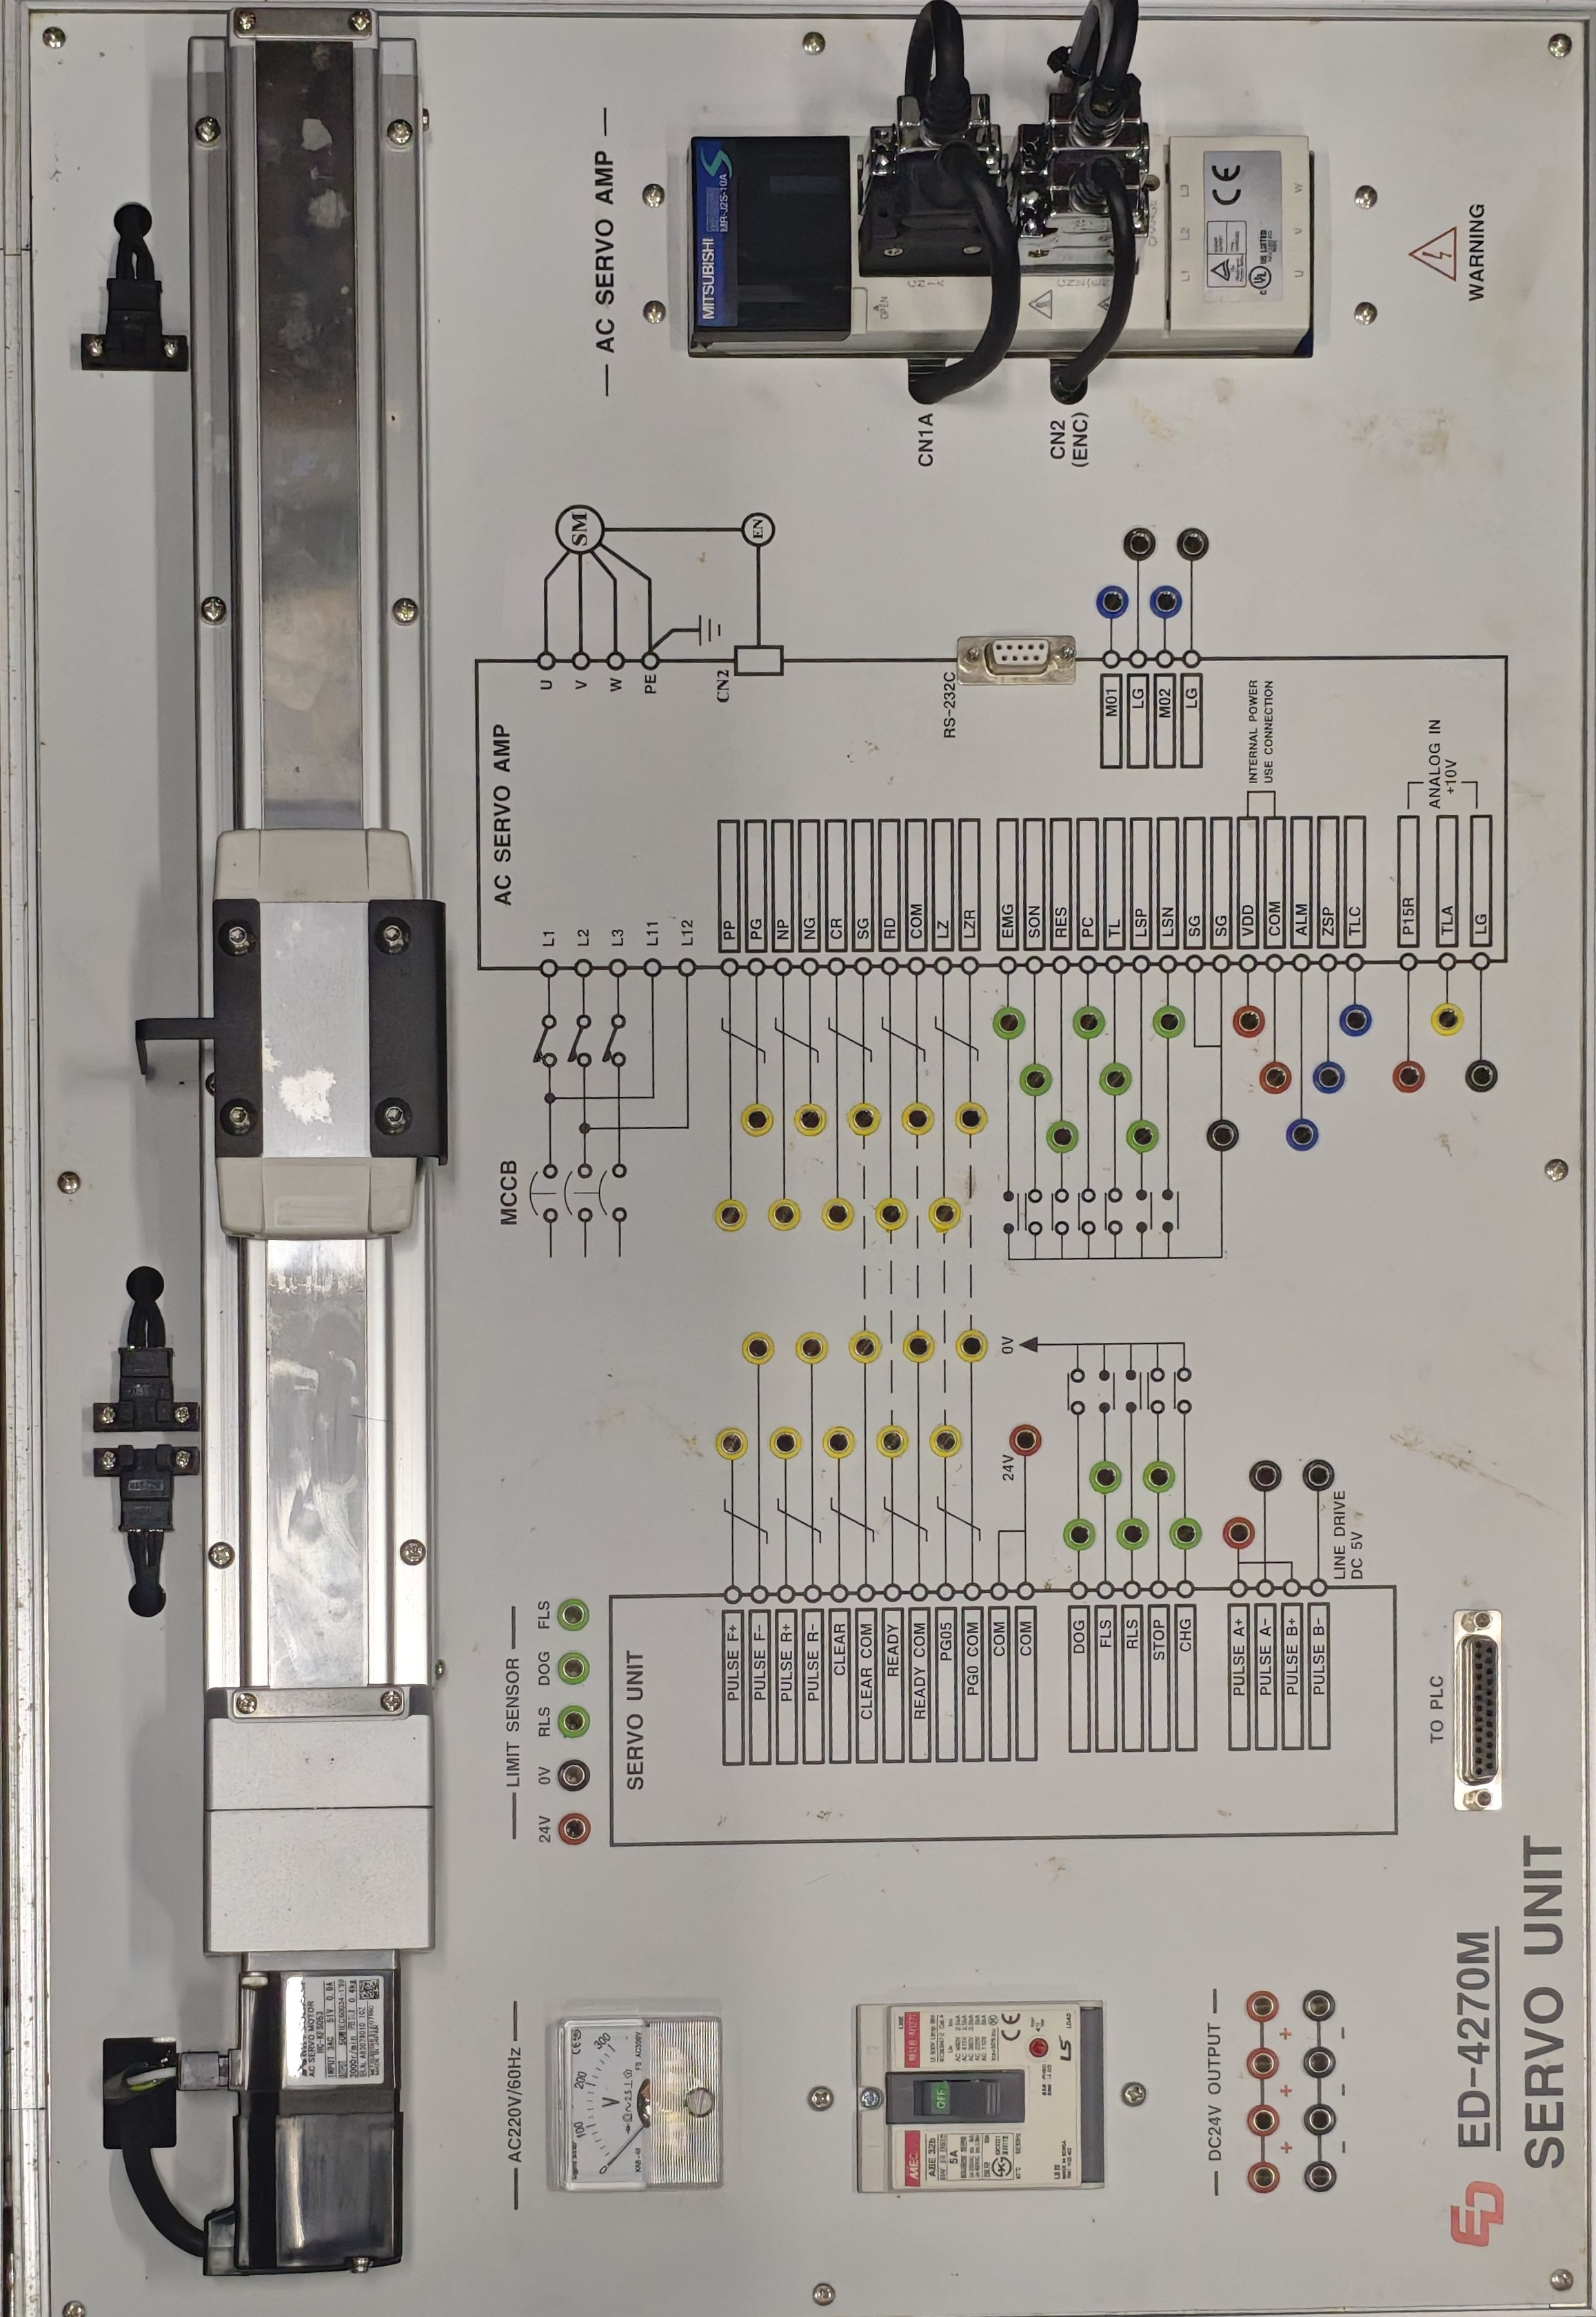
\includegraphics[width=0.4\textwidth, angle=-90]{Gambar/ED-4270m.jpg}
    \caption{Modul Laboratorium ED4270m}
    \label{fig gambar2_bab1}
\end{figure}

Kendati menawarkan performa mekanis yang superior, implementasi algoritma
\textit{S-Curve} pada sistem tertanam (\textit{embedded system}) memiliki
kendala komputasi yang signifikan. Persamaan matematis pembentukan lintasan
\textit{S-Curve} melibatkan kalkulasi polinomial orde tiga, operasi kuadratik,
dan pembagian pecahan secara simultan yang harus diselesaikan dalam orde
mikrodetik. Jika kalkulasi berat ini dibebankan pada mikrokontroler standar
berinti tunggal (\textit{single-core}), siklus interupsi pembawa pulsa menuju
\textit{driver} servo akan terganggu, memicu terjadinya \textit{jitter} sinyal
yang merusak akurasi posisi. Oleh karena itu, penggunaan arsitektur
mikrokontroler \textit{dual-core} menjadi solusi esensial dalam penelitian ini,
di mana beban kerja dibagi secara deterministik: \textit{Core 0} didedikasikan
penuh untuk kalkulasi matematika profil pergerakan dan komunikasi data,
sedangkan \textit{Core 1} berfokus tanpa interupsi untuk membangkitkan rangkaian
pulsa kecepatan tinggi secara presisi.

Selain stabilitas komputasi pengontrol, integritas transmisi sinyal dari
mikrokontroler menuju \textit{Servo Amplifier} MR-J2S-10A juga memegang peranan
krusial. Sinyal pulsa berkecepatan tinggi berfrekuensi tinggi rawan terdistorsi
oleh interferensi elektromagnetik akibat induksi medan magnet motor dan
pensaklaran inverter internal \textit{servo amplifier}. Penggunaan pengkabelan
berpasangan terpilin yang digerakkan oleh sirkuit terintegrasi
\textit{differential line driver} merupakan syarat mutlak untuk menjamin
kestabilan pengiriman pulsa kontrol tanpa kehilangan data. Sebagai solusinya,
sirkuit antarmuka \textit{differential line driver} diintegrasikan guna mengubah
sinyal pulsa menjadi sepasang sinyal diferensial berstandar RS-422, sehingga
gangguan elektromagnetik dari lingkungan luar dapat diredam sepenuhnya melalui
mekanisme penolakan modus bersama \textit{(common-mode rejection)} di sisi
penerima amplifier servo.

Guna membuktikan validitas performa peredaman getaran dari algoritma
\textit{S-Curve} yang dirancang terhadap metode konvensional, penelitian tugas
akhir ini mengintegrasikan sebuah metode pengujian eksperimental berupa
\textit{liquid slosh control} (pengendalian riak cairan). Dengan menaruh wadah
berisi cairan di atas meja geser \textit{linear stage} modul ED4270m,
efektivitas peredaman efek sentakan mekanis dari profil \textit{rectangular},
\textit{trapezoidal}, dan \textit{S-Curve} dapat diamati secara empiris dan
visual melalui stabilitas permukaan cairan serta riak gelombang yang terbentuk
selama fase akselerasi dan deselerasi.

\section{Perumusan Masalah}
Berdasarkan deskripsi mendalam pada latar belakang di atas, rumusan masalah dalam penelitian tugas akhir ini dirancang sebagai berikut:
\begin{enumerate}
    \item Bagaimana memodelkan persamaan matematis orde tiga dan mengimplementasikan arsitektur kode program pemisahan tugas (\textit{multitasking dual-core}) untuk membangkitkan profil pergerakan \textit{rectangular, trapezoidal}, dan \textit{S-Curve} secara \textit{real-time}?
    \item Bagaimana merancang sirkuit antarmuka perangkat keras berbasis \textit{differential line driver} guna menjaga integritas transmisi sinyal pulsa kendali frekuensi tinggi menuju \textit{servo amplifier} Melservo-J2-Super?
    \item Bagaimana hasil perbandingan kinerja empiris dari ketiga profil pergerakan tersebut ditinjau dari parameter respons \textit{settling time}, \textit{positional error} via \textit{encoder feedback}, serta tingkat osilasi permukaan air pada metode pengujian \textit{liquid slosh control}?
\end{enumerate}

\section{Pembatasan Masalah}
Agar arah penelitian tetap fokus dan terukur sesuai dengan target kompetensi, batasan masalah ditetapkan sebagai berikut:
\begin{enumerate}
    \item Validasi eksperimental dan pengambilan data dinamis murni dilakukan menggunakan unit perangkat keras laboratorium berupa Modul Mekatronika ED4270m (\textit{AC Servo Linear Stage Unit}) dengan penambahan beban uji eksternal berupa wadah berisi cairan.
    \item Perangkat keras aktuasi dibatasi pada unit \textit{Servo Amplifier} Mitsubishi Melservo-J2-Super tipe MR-J2S-10A beserta unit motor servo AC internal bawaan modul ED4270m.
    \item Parameter performa yang diukur dan dianalisis secara komparatif dibatasi pada aspek kinematika gerak aktuator meliputi akurasi target posisi, deviasi \textit{positional error}, durasi \textit{settling time}, serta dokumentasi visual riak cairan, tanpa mencakup kalkulasi efisiensi konsumsi daya listrik maupun disipasi termal pada motor.
    \item Unit mikrokontroler \textit{dual-core} bertindak sebagai pusat kendali level rendah (\textit{low-level controller}) untuk kalkulasi algoritma lintasan dan generator pulsa, sedangkan pengiriman parameter penargetan awal (\textit{setpoint}) dilakukan melalui koneksi serial komputer.
\end{enumerate}